\subsection{Projektstrukturplan}

Ein größeres Projekt umzusetzen erfordert viel Arbeit. Manchmal erscheinen die Aufgaben so komplex, das man nicht weiß wo man zuerst anfangen soll. Um Arbeit und konkrete Arbeitsschritte besser darstellen zu können, greifen Projektmanager:innen oftmals auf den Projektstrukturplan zurück. Der Projektstrukturplan teilt größere und komplexere Arbeiten in kleine und konkrete Arbeitspakete auf. Die konkreten Arbeitspakete werden anschließend gruppiert, sequenziell nummeriert und den verschiedenen Abteilungen bzw. Mitarbeiter:innen zugeteilt. Anhand eines Projektstrukturplans kann ein Gantt Plan erstellt werden. Der Gantt Plan zeigt die zeitliche Abfolge der einzelnen Arbeitspakete. Der Projektstrukturplan ist ein wichtiges Werkzeug für die Planung und Steuerung von Projekten. In Abbildung \ref{fig:projektstrukturplan} wird der Projektstrukturplan des Prototypen dargestellt.

\begin{figure}[H]
  \centering
  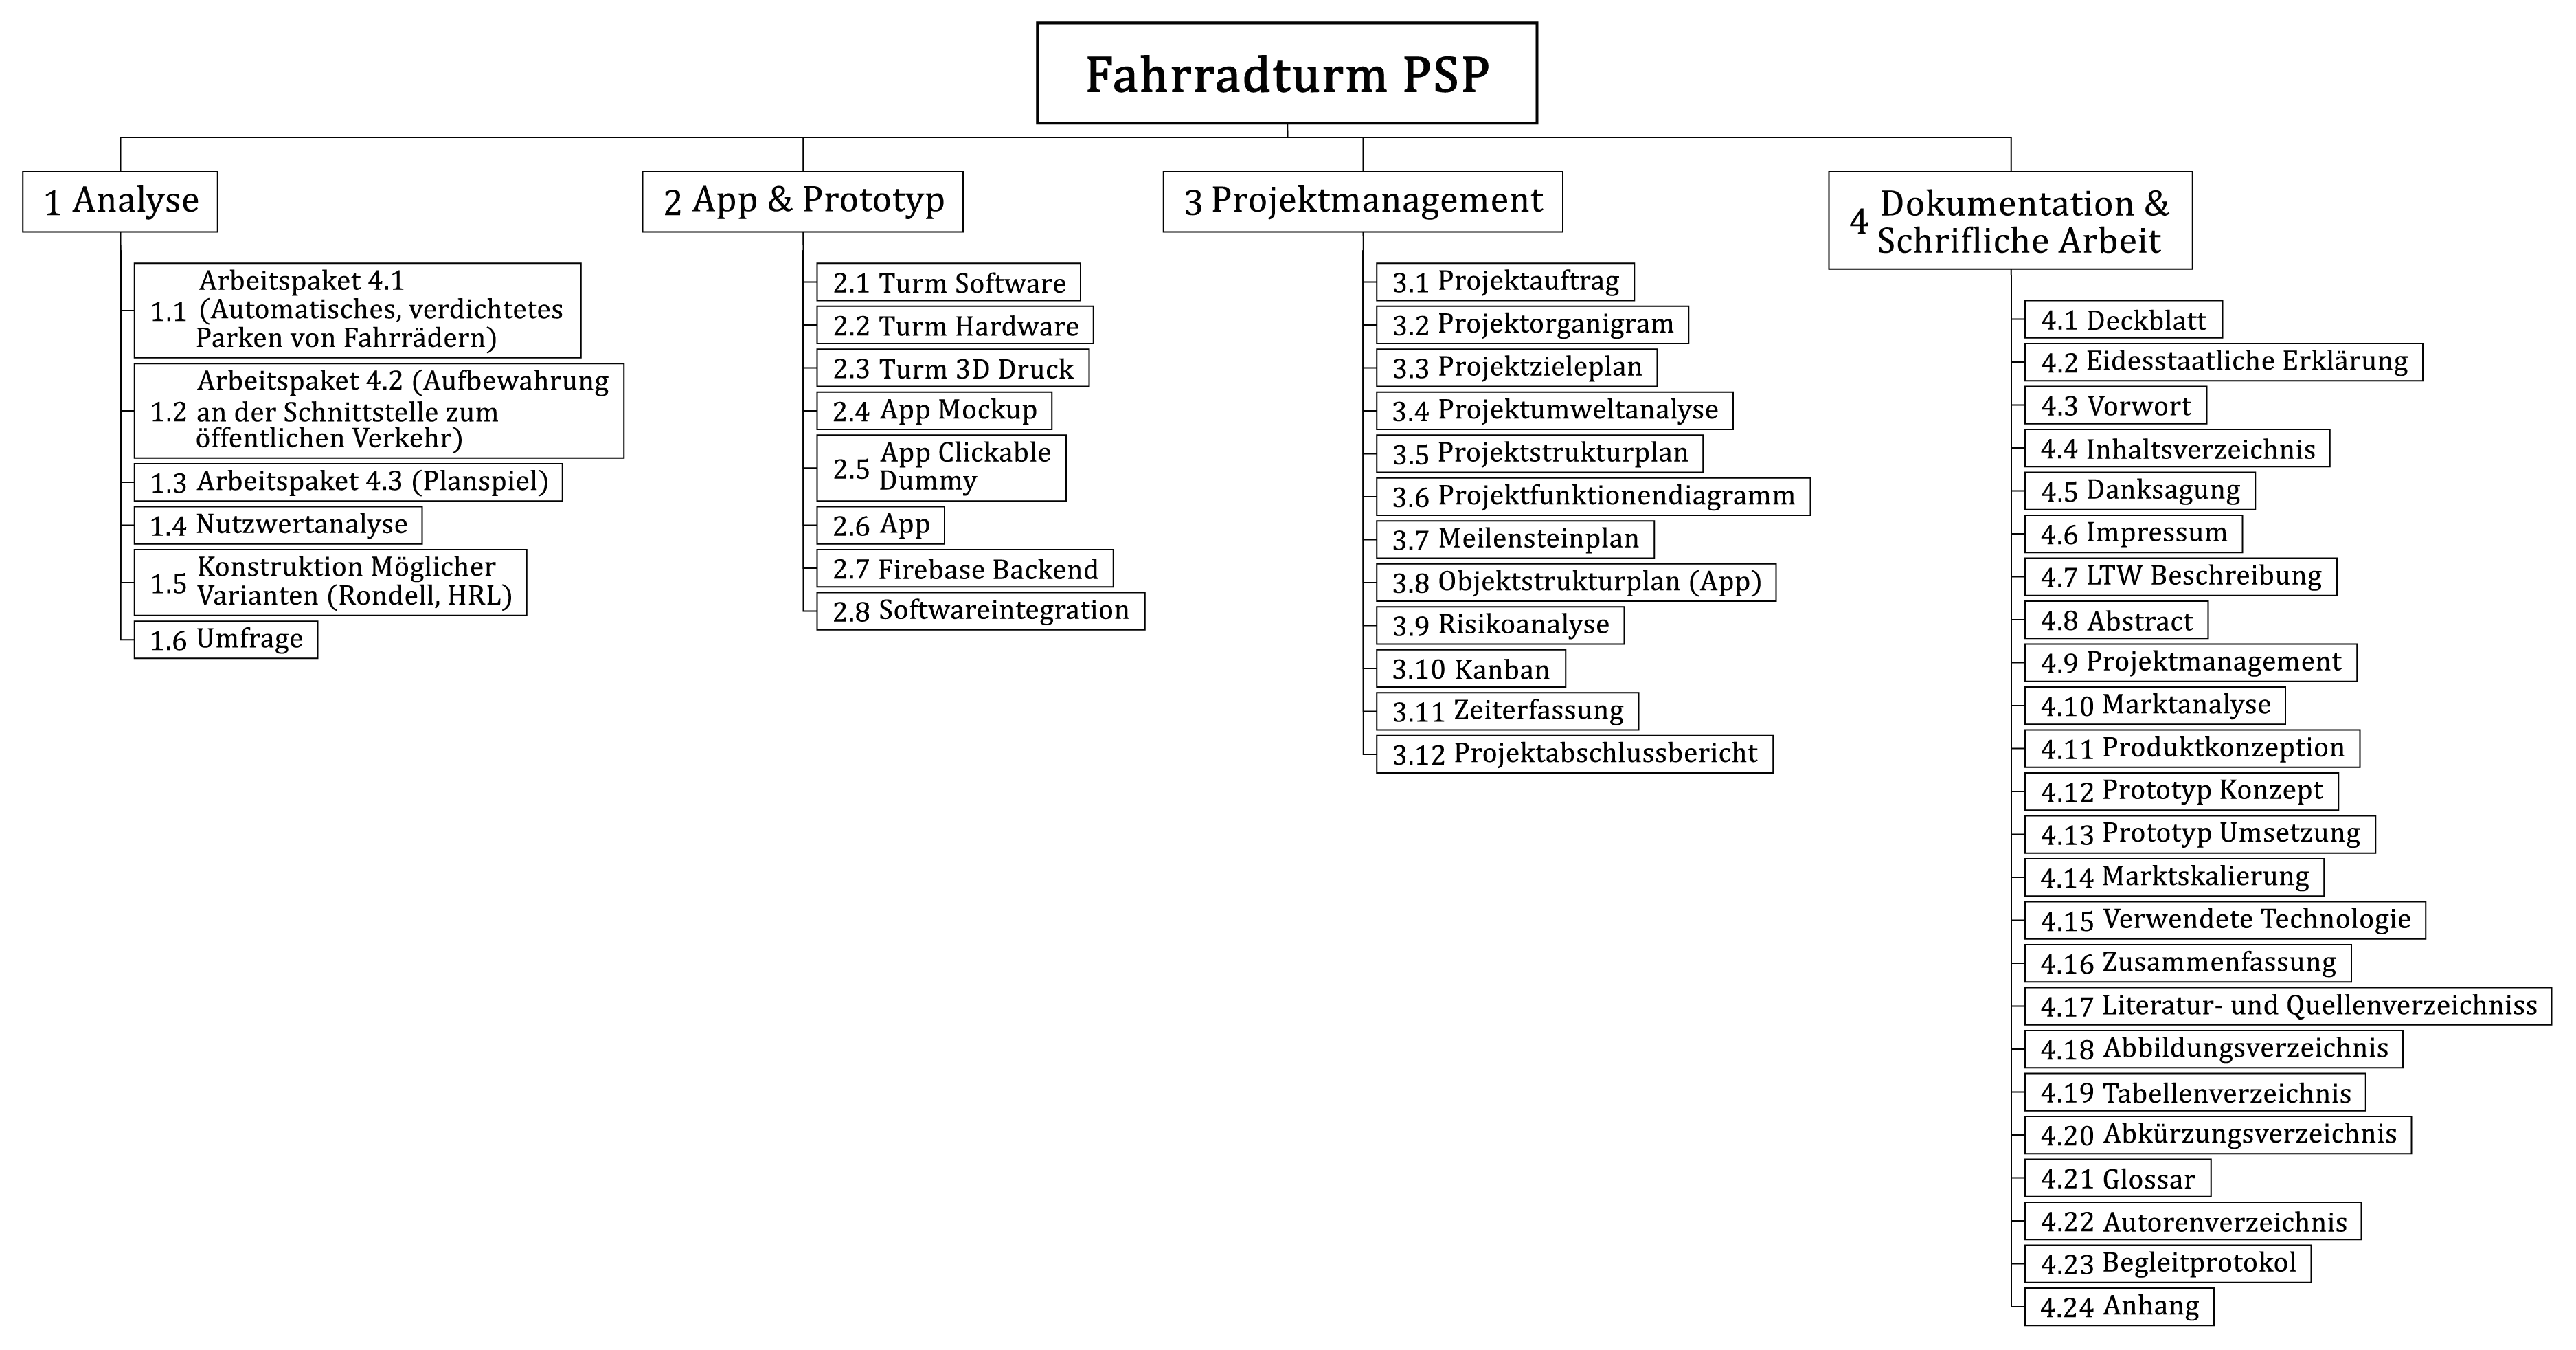
\includegraphics[width=1\textwidth]{images/projektstrukturplan}
  \caption{Projektstrukturplan}
  \label{fig:projektstrukturplan}
\end{figure}
